\lettrine[lines=2, findent=3pt,nindent=0pt]{T}{ypically}, one has not access to the density matrix of the system been used for metrology or for other quantum process.
Moreover, for systems on which the particle number is very large, this is the case when one wants to do metrology with quantum states, the details of the density matrix are forbidden by practical reasons.
Since the quantum Fisher information is based on the complete knowledge of the density matrix, shortcuts to avoid the complete tomography must be developed as we have had shown one practical case on the previous chapter.
In this chapter, we obtain a general procedure to get an optimal bound for the quantum Fisher information based on as many expectation values of the initial state as one is ready to measure.
Two main features are worth to mention again.
First, in general this method gives us an optimal tight bound.
Last but not least, the bound is based on the expectation values of the initial state only, so it is not necessary to perform an evolution of the state to estimate how well will it behave.
This is in contrast to other approaches one can find in the literature, an it is a time saving concept.

The figure of merit of bounds from below for the quantum Fisher information based on expectation values of the initial state is the following,
\be
  \mathcal{F}_{\text{Q}} [\rho,J_z] \geq \frac{\expect{J_x}^2}{\varian{J_y}}.
\ee
where the state is polarized along the $Ox$-axis and the variance of the $J_y$ operator is smaller than the standard.
On the previous chapter we also have shown one of these bound specifically designed for unpolarized Dicke states.

Homogeneous magnetometry, $\bs{B} = B\bs{k}$ where $B$ is constant in time.

Section~[REF], see magnetometry, generator $J_z$.

Quantum Fisher information $\mathcal{F}_{\text{Q}} [\rho, J_z]$.

\subsection{Minimum of a convex funtion of the states based on the expectation values}

Convex function of states, $g(\rho)$.

Which is the lowest possible value of $g(\rho)$ for a state where some expectation values of $\{W_{i}\}_{i=0}^M$ operators, $w_i = \tr(\rho {W}_i)$ are known?

Such bound is defined,
\be
  g(\rho) \geq \mathcal{B}_{g}(w_1,w_2,...)
\ee

For this purpose we use simplify our discourse to one observable or equivalently one parameter, $w = \tr(\rho W)$ and formally the bound is defined as follows,
\be
  g(\rho) \geq \big\{ \mathcal{B}_{g}(w) := \min_{\rho}  g(\rho) \;|\; w = \tr(\rho W)\big\}.
\ee

The bound from below of such a funtion $g(\rho)$ is convex too [NEED TO BE SHOWN?].

Therefore, we use the Legendre transform to get rid out of the state and still keep all the necessary information to reconstruct the $\mathcal{B}_{g}$ bound.
\be
  \hat{g}(r) = \sup_{\rho}\{ r\expect{W}_{\rho}-g(\rho)\}
\ee

Now we have the Legendre transform, we recover the bound from below of $g(\rho)$ as
\be
  \mathcal{B}_g (w) = \sup_{r}\big\{rw-\sup_{\rho}\{r\expect{W}_{\rho}-g(\rho)\}\big\}
\ee


\be
  \mathcal{B}_{\mathcal{F}}(w_1,w_2,...)
\ee

\begin{figure}
  \centering
  \igwithlabel{(a)}{scale=.65}{img/plots/LT_fidGHZ.pdf}
  \igwithlabel{(b)}{scale=.65}{img/plots/LT_fidDicke.pdf}
  \caption{(a) Analytical solution of the bound $\mathcal{B}_{\mathcal{F}}$ for different values of the fidelity with respect to the GHZ state. (b) Numerical results for the minimum quantum Fisher information as a function of the fidelity with respect of unpolarise Dicke states perpendicular to the magnetic field, $|\text{D}_N^0\rangle$. (blue-line) For systems with 4 particles and (red-dashed) for system with 8 particles. One may notice that when the fidelity is at its maximum the bound approaches to 0.5 as it is the quantum Fisher information for large particle number.}
  \label{fig:vd-secuence-evo}
\end{figure}

\begin{figure}
  \centering
  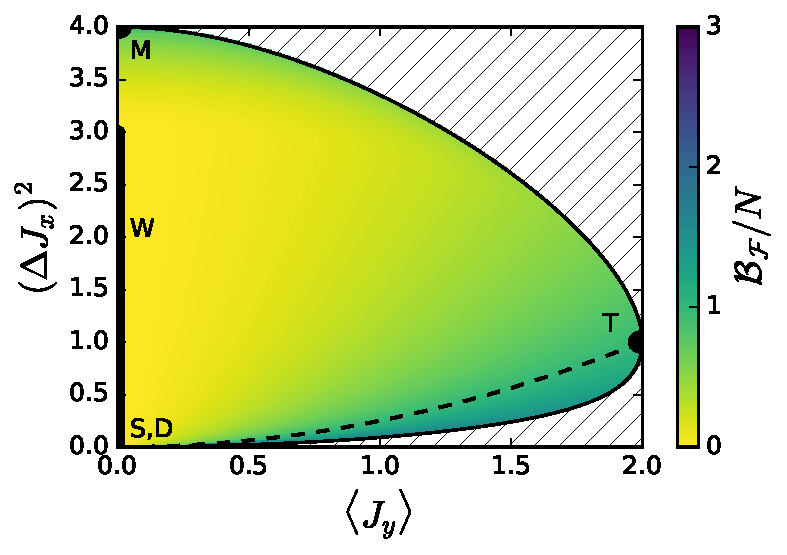
\includegraphics[scale=.65]{img/plots/LT_spsq2d_4.pdf}
  \caption{(dashed) Boundary for the SQL, all points above the line achieve semi-classical precisions, while the points below the line achieve better precisions than with classical systems.}
  \label{fig:vd-secuence-evo}
\end{figure}

\begin{figure}
  \centering
  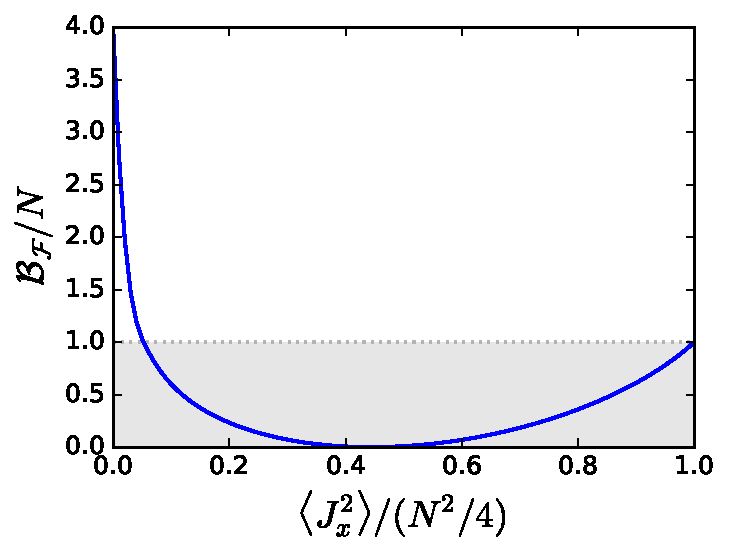
\includegraphics[scale=.65]{img/plots/LT_dicke_edge.pdf}
  \caption{}
  \label{fig:vd-secuence-evo}
\end{figure}

\begin{figure}
  \centering
  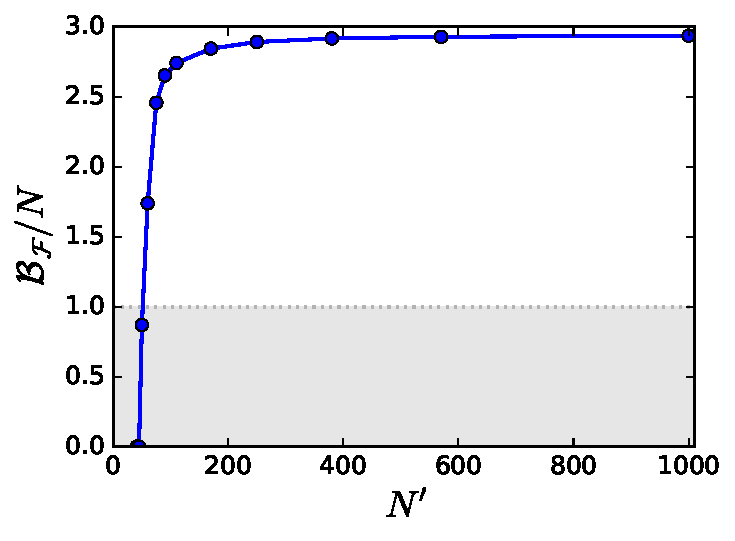
\includegraphics[scale=.65]{img/plots/LT_dicke_7900_asymp.pdf}
  \caption{Secuence of the evolution of an unpolarized Dicke state of 16 qubits for $\Theta=\{i\pi/6\}_{i=0}^4$. Bloch spheres representing the Hirusi distribution of the state, and below PDF of the $J_x$ POVM for each step of the secuence}
  \label{fig:vd-secuence-evo}
\end{figure}
